% written by scripts/reuse_short.py from the sources of the short paper; do not edit
In the final design each job gets one fresh container: no network, no capabilities, a seccomp filter, a read-only root, an unprivileged user, 2 CPUs, 10 GiB of memory, 4,096 processes, and temporary filesystems capped in bytes and inodes. The only request channel is a per-job Unix socket to a forwarder, which passes only chat-completion requests with allow-listed fields, text-only content and an approved template hash, under rate and size caps. Agent runs start only if eight recorded hashes (image, code, flags, model files) still match.

A \emph{canary} is a scripted attack with a machine-checked outcome.

\begin{table}[!tb]
\centering
\caption{Runner versions.}\label{tab:versions}
\footnotesize
\begin{tabular}{@{}
  >{\raggedright\arraybackslash}p{(\linewidth - 4\tabcolsep) * \real{0.2000}}
  >{\raggedright\arraybackslash}p{(\linewidth - 4\tabcolsep) * \real{0.1900}}
  >{\raggedright\arraybackslash}p{(\linewidth - 4\tabcolsep) * \real{0.6100}}@{}}
\toprule
\begin{minipage}[b]{\linewidth}\raggedright
Runner version
\end{minipage} & \begin{minipage}[b]{\linewidth}\raggedright
Canaries passed
\end{minipage} & \begin{minipage}[b]{\linewidth}\raggedright
Security findings of independent verifiers
\end{minipage} \\
\midrule
1. Container per command & 52/52 & 4 high: host-side install ran the agent's \texttt{setup.py} (builder-found); symlink leaked a host file; 10 GiB of host disk reserved in 0.005 s; host copied a sparse file in full \\
2. Hardened, per command & 60/60 (57/60 before canary fixes) & 4 high, 1 untested: host overwrote a file through a planted link; cleanup followed links; 6 GiB reserved in 0.012 s; 200,000 files in 2.4 s \\
3. Container per job & 98/98 & 1 high: the model server could fetch URLs named in requests; 2 medium \\
4--6. Request filter added, tightened & 134/134, 159/159, 191/191 & medium at most \\
7. Final & 200/200 & no high or medium \\
\bottomrule
\end{tabular}
\end{table}

\begin{figure}[!tb]
\centering
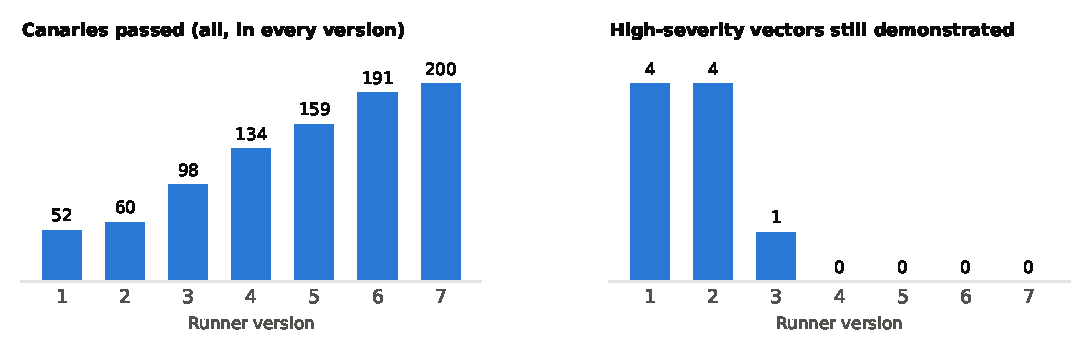
\includegraphics[width=\linewidth]{fig/runner_versions.pdf}
\caption{Canaries passed and high-severity vectors found, per runner version.}
\label{fig:versions}
\end{figure}


\paragraph{Passing canaries proved little.} No attack escaped the container's namespaces or privileges in any round. Nine demonstrated high-severity vectors came through what the host shared with it: host-side steps that touched agent-written files, resource limits (a known class \citep{gao2019houdini}) and the model server.

\paragraph{Final version.} Controls on 481 tasks (reference patch 481/481, empty patch 0/481) showed no verdict, exit-code or test-summary difference from the previous version. After the runner was killed, the container was gone within 149 s with no further model request. The final runner completed a 24-job list at 251--254 runs per hour with 8 workers.

\paragraph{What remains.} Containers share the host kernel; user namespaces are not remapped; the request parser runs in the trusted runner; a job can slow others through the shared model server within its caps. Our claim is conditional: against the stated adversary and with the eight hashes matching, no tested attack succeeded.
